%Chapter 5 - Evaluating the MEGA65 project against known risks
%

\chapter{Evaluating the MEGA65 project against known risks}
\label{Chapter5}
This chapter aims to provide useful advice to the MEGA65 project with the aim of reducing the project's risk. To achieve this, the detailed snapshot of the project's progress at the point in time of July 2018, chapter \ref{Chapter4}, is evaluated to determine its risk levels in the known risks identified in the case studies in chapter \ref{Chapter3}. The layout of this chapter is that each risk identified in the risk list is given a section and within each section the MEGA65 project is scrutinised to determine its risk level to that specific risk. At the end of the chapter a conclusion is drawn on the MEGA65 project's risk level as of July 2019. For the identified high risk areas, some advice that could reduce the project's risk level is given. This advice is in the form of alternate solutions or methods of doing things and their potential risk reduction. The risks to the MEGA65 project are determined by following the guidelines given in \textit{AS ISO 31000:2018 Risk management — Guidelines} 
\cite{RN164} and categorised using the definition of damage listed in the table at the start of chapter \ref{Chapter3}. The risk is determined using the risk matrix figure \ref{riskmatrix}.

\begin{figure} \begin{center}
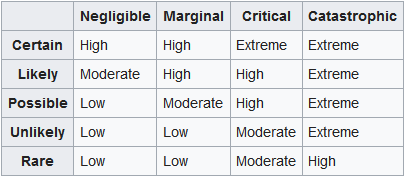
\includegraphics[width=.3\linewidth]{pics/riskmatrix} 
\end{center} 
\caption{Risk matrix showing levels of risk for given likelihood and harm severity.\\}
\label{riskmatrix}
\end{figure}

%----------------------------------------------------------------------------------------
%----------------------------------------------------------------------------------------
\section{Law and Regulations}
The MEGA65 products, the MEGAphone and the desktop version, will have to comply with the relevant laws and regulations of the countries in which they are sold in. These laws and regulations are specific to each country, but the general definition and intent of the laws and regulations is similar in lots of places around the world, at least in regard to electronic consumer products. This similarity in laws and regulations comes, in part, from international organisations and standards being adopted or used as a starting point for country specific standards. While the potential damage to a project is catastrophic as it could force a project to be abandoned in the most extreme cases, the uncertainty is fairly low as the laws and regulations are placed in the public domain before being enacted and should be unambiguous. Two cases of laws and regulations causing problems where identified during the case studies. The Raspberry Pi was delayed due to electronic interference testing and the Spectrum Vega was delayed due to age rating testing. While both of these examples are European specific, they similar nature of the laws and regulations of many market places make them relevant for a large portion of the world. \\

The MEGA65 project is rated as a marginal level of damage to the project from a law and regulation related risk. This is due to the projects ability to adapt to change quite well and it doesn't have a strict time or cost constraints. If a product was found to breach electronic interference laws for example, the MEGA65 team would be able to redesign and test the new product with only marginal delays in time and cost. The MEGA65 team is aware of this risk and of the most notable examples of these laws, such as electronic interference and age rating testing, but not of the specific laws of each market they are intending to operate in. The project has indicated that they are intending to carry out specific research into the laws and regulations of certain markets. Until this research has been conducted, the project has been rated at a likely level of probability of occurring. 

Likelihood - Likely  
Potential damage - Marginal
Risk - High


\subsection{Brexit-like events}
There are no foreseeable Brexit-like events that would be likely to affect the MEGA65 project. Brexit itself is unlikely to affect the MEGA65 project as the project is largely based in Australia, with the desktop version being made in Germany. The potential market for the MEGA65 in the United Kingdom is small and there will likely be some level of agreement with current laws and regulations within the United Kingdom to reduce to the disruption to the market during the transition out of the EU. The project has been rated as unlikly to experience this type of risk. The potential damage to the MEGA65 project was rated as marginal.

Likelihood - Unlikely
Potential damage - Marginal
Risk - Low


\section{Project Constraints}
The MEGA65 project is not bound to tight constraints on project cost. The desktop form factor may be subject to more tight constraints but overall the project was started as a hobby and continues in part as a learning tool for students at Flinders University. The funding model is also largely not dependant on selling the product to generate a profit. The MEGA65 project is then rated as a unlikely probability of occurring and a marginal risk.

Likelihood - Unlikely
Potential damage - Marginal
Risk - Low


\section{Crowd-funding}
The MEGA65 is considering using crowd-funding to raise funds but importantly they will wait until the design and component selection is complete before launching the campaign.

\subsection{Contract of sale}
The fact the the MEGA65 team are waiting until much later in the productisation process to launch the crowd-funding campaign greatly reduces the risks associated with it. The risk comes from forming a contract of sale between MEGA65 project and backers of the crowd-funding campaign and that contract not being fur filled. This could lead to legal proceedings against the MEGA65 project. The fact that the MEGA65 project won't do this until a much later stage in productisation means the chance that the MEGA65 project will fail to deliver the product is greatly reduced. This is due to the uncertainty factor being reduced as a lot of the design and component selection is done as such is not uncertain but certain. The mega65 is rated as a an unlikely probability that it would cause a critical amount of damage to the project.

Likelihood - Unlikely
Potential damage - Critical
Risk - Moderate


\subsection{Currency}
If the MEGA65 team does decide to go the crowd-funding route they will need to decide on what currency to operate in. The risk here is the currency exchange rate drops after receiving the funds and now the actual purchasing power of the funds may be reduced. This risk is increased with time, the longer you hold onto the funds without spending them the more chance the exchange rate will fluctuate. As the MEGA65 team will wait until the product is much further along in the productisation process before crowd-funding this time period will be significantly reduced. There are also some currency which are more stable, in general, and research into these would also reduce the risk by allowing the MEGA65 team to use a stable currency to raise funds in. Another aspect to consider is the currency in which the majority of the funds will be spent i.e. if most of the parts and components are coming from USA companies then it may make sense to use the USD as the crowd-funding currency. The MEGA65 project is rated as unlikely to experience these risks and it would most likely produce a marginal level of damage if it did occur.

Likelihood - Unlikely
Potential damage - Marginal
Risk - Low


\subsection{Failure to meet goal}
Due to the funding model of the MEGA65 project


\section{Sourcing old components}
MEGA65 plans to use floppy drives, mention this in chapter 4 too!


\section{Use of 3rd party intellectual property}
This is the main problem area:
- MEGA65 wanted to use a Commodore logo on the Commodore keyboard key
ask Paul if they had agreement to use commodore icon
recommend they don't use Commodore icon but a similar design

- MEGA65 NEEDS to use BASIC ROM/s to function as a Commodore compatibly computer
ask paul if they have agreement
recommend they don't use 3rd party BASIC ROM and consider producing their own

- games and applications licence

\section{Open-source business}
ask paul about business model


\section{Loss of intellectual property}
ask paul who holds rights to everything mega65 related inc. software designed by students, FPGA, firmware and PCB designs. desktop version too, case CAD, keyboard design, PCB


\section{Supplier failure}
zask paul about suppliers, check skype for desktop form factor supplier, make risk assessment on them



\section{Open-source fair use}
should not be a concern for MEGA65

ask paul if they used any open-source components


\section{Physical production problems}
